% Description section, to be included in RASD.tex

\section{Overall Description}
\label{sect:overview}

\subsection{Product perspective}
The application's users will be able to interact through either mobile apps or web-based applications (predominantly with an interface optimized for mobile devices).

When used by customers, the system will need to use a web mapping service such as Google Maps to provide a position (if needed) and calculate travel times.

On the other hand, when used in stores, it will need to be connected to QR code readers (either mobile devices or dedicated scanners) ticket printers, and screens.

% Scenarios file, to be included in overview.tex

\subsubsection{Scenarios}
The following scenarios are provided to describe possible situations during the usage of CLup.

\paragraph{Scenario 1}
Nathan, during the pandemic, needs a way to safely go grocery shopping, avoiding long queues out of supermarkets. His friend John suggests him to download the CLup app to line up from home; Nathan is intrigued and immediately downloads it, signs up and enqueues for his favorite shop.

\paragraph{Scenario 2}
After being enqueued for about thirty minutes, Nathan receives a notification telling him his turn is close and he needs to leave home. After reaching the supermarket he waits for some minutes until his number gets displayed by the shop; he then passes the QR code shown by the application at a scanner and enters the shop. Once he has done, he scans again the code at the exit and goes home. 

\paragraph{Scenario 3}
Ms. Margareth is not accustomed to technology, so she does not use a smartphone; as she needs to go grocery shopping, she goes directly to the store and gets a physical ticket, so she can wait outside with few people, as most use CLup. Once she sees her number is reached, she scans the ticket and enters.

\paragraph{Scenario 4}
Nathan knows Julie, the owner of a bakery close to his house, so he tells her about CLup. She is curious and downloads the app, registering her shop. She then logs in as Store Manager into the tablet she uses for work, so that her employees can use it to scan codes and monitor the entrance of customers.

\paragraph{Scenario 5}
Anthony works for a supermarket that adopted CLup. As a store manager, he has the duty of keeping updated the store’s inventory and make customers respect their turns. Luckily, the store decided to install some QR code readers connected to CLup at entrances, so he doesn’t have to scan every customer’s code himself. 

\paragraph{Scenario 6}
As Joe had some free time, he decided to get a physical ticket for the supermarket, hoping few people were already lined up. After 10 minutes of being enqueued he receives an important call and needs to leave; he decides to scan his ticket to dequeue and let the people behind him enter some time before.

\paragraph{Scenario 7}
Andrew is at home, waiting for his turn after he requested a ticket. Suddenly he receives a notification from CLup, letting him know that someone in front of him dequeued and giving him the possibility to enter earlier than expected. He gladly accepts and gets ready to go.

\paragraph{Scenario 8}
Anastasia knows she needs to go shopping for groceries the next day but has a very tight schedule. Luckily, she can use CLup to book a visit for the exact time she chooses, so she requests a reservation. The next day she can enter without having to line up, thus saving much of her time.

\paragraph{Scenario 9}
Confident about his free time, Nick booked three visits for the next week. The day before the second one he remembered he was actually busy, so he logged in the application and canceled the reservation.

\subsection{Product functions}
The major objective of the application is to decrease queues outside stores; this is achieved by allowing customers to line up from home and book visits for specific dates and times. These functions are integrated with alerts telling the user when to leave home, along with possibility to subscribe to notifications about store occupancy throughout the week to better plan store visits.

For customers not using the application, options to take physical tickets and wait outside store are offered.

\subsection{User characteristics}
Due to the nature of the application, users can span a wide variety of people with different needs of accessibility and functions.

\subsubsection{Actors}
Actors represent the groups of people that interact with the application. The relations among the active actors are shown in Figure \ref{actors}.
\begin{itemize}[itemsep=-1mm, topsep=-1mm]
	\item \textbf{Prospective e-Customer}: A person who would like to use the application as customer
	\item \textbf{Prospective Store Manager}: A person who would like to register their store
	\item \textbf{Physical Customer}: A customer not registered to the application
	\item \textbf{e-Customer}: A customer using the application
	\item \textbf{Store Manager}: A user managing a store
\end{itemize}

\begin{center}
	\begin{figure}[h]
		\centering	
		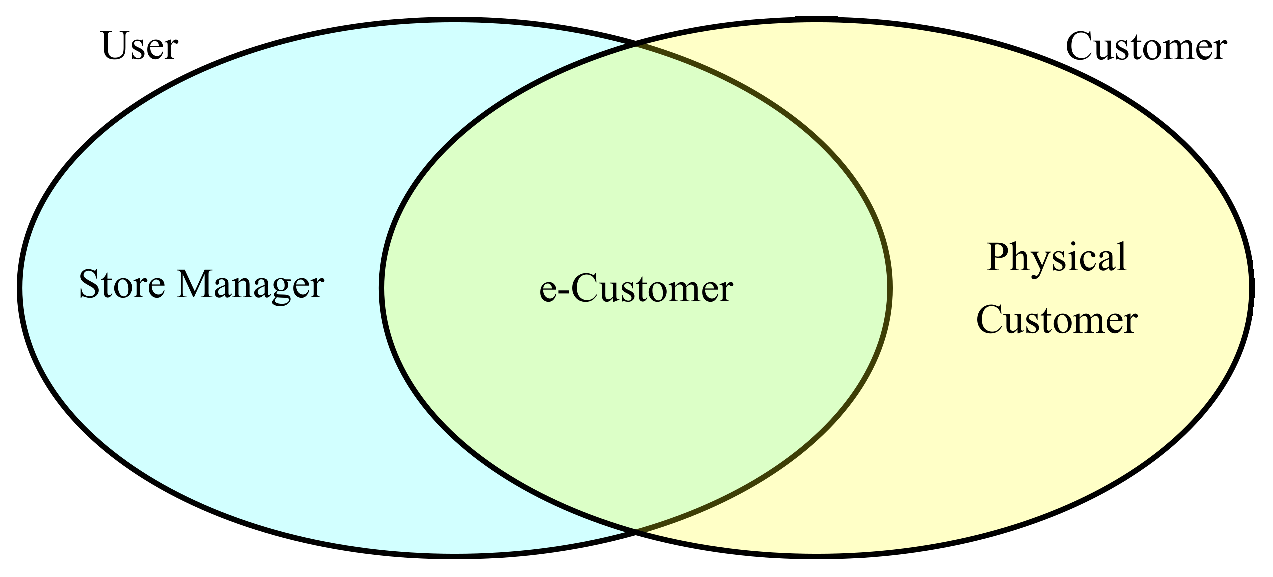
\includegraphics[width=.7\textwidth] {actors}
		\caption{Active actor relations}
		\label{actors} 
	\end{figure}
\end{center}

\subsection{Assumptions, dependencies and constraints}

\subsubsection{Text assumptions}
Due to the ambiguity created by the natural language, we made the following assumptions about the specification.

\begin{itemize}[itemsep=-1mm, topsep=-1mm]
	\item For each store exists only one store manager; this way, if more people need to use the functions they will need an already logged in terminal
	\item Some places in stores will need to be reserved to tickets, both in their physical and virtual form, to avoid creating situations where reservations monopolize the entrances
	\item QR codes will need to be scanned both at entrance and exit, in order to better know the store's occupation and how much time customers spend inside
\end{itemize}

% File for domain assumptions, to be included in overview.tex

\subsubsection{Domain assumptions}

\begin{itemize}[itemsep=-1mm, topsep=-1mm]
	\item [\textbf{[D0]}] Prospective users will complete the registration process
	\item [\textbf{[D1]}] Only people enqueued access the stores (both app and physical)
	\item [\textbf{[D2]}] Information provided by e-customers corresponds to their will
	\item [\textbf{[D3]}] Information provided by users upon registration is correct
	\item [\textbf{[D4]}] Customers enter only if allowed by the application
	\item [\textbf{[D5]}] Customers respect the choices made during a ticket creation or while booking a visit
	\item [\textbf{[D6]}] Calculated travel time is correct
	\item [\textbf{[D7]}] Information about stores inserted by SMs is correct
	\item [\textbf{[D8]}] Customers entering a store exit after some time
	\item [\textbf{[D9]}] If a client exits at a given time, he must have entered in the same opening period
	\item [\textbf{[D10]}] Ticket printers and QR readers work properly
	\item [\textbf{[D11]}] The internet connection is always working
	\item [\textbf{[D12]}] Users accept to receive notifications from the application
	\item [\textbf{[D13]}] Stores show the current customer number
	\item [\textbf{[D14]}] The external web mapping system is always available and there is signal
\end{itemize}

\newpage
\subsection{Domain Diagrams}
The high-level class diagram of the application can be seen in Figure \ref{class}, while Figure \ref{ticket_state} contains the state diagram for tickets; the beginning of the $CanEnter$ state corresponds to the start of the delay window. Figure \ref{open_store} shows the acceptance states of a store during its opening hours.

\begin{center}
	\begin{figure}[h]
		\centering	
		\includegraphics[width=0.9\textwidth] {state_diagrams/ticket}
		\caption{Ticket state diagram}
		\label{ticket_state} 
	\end{figure}
\end{center}

\begin{center}
	\begin{figure}[h]
		\centering	
		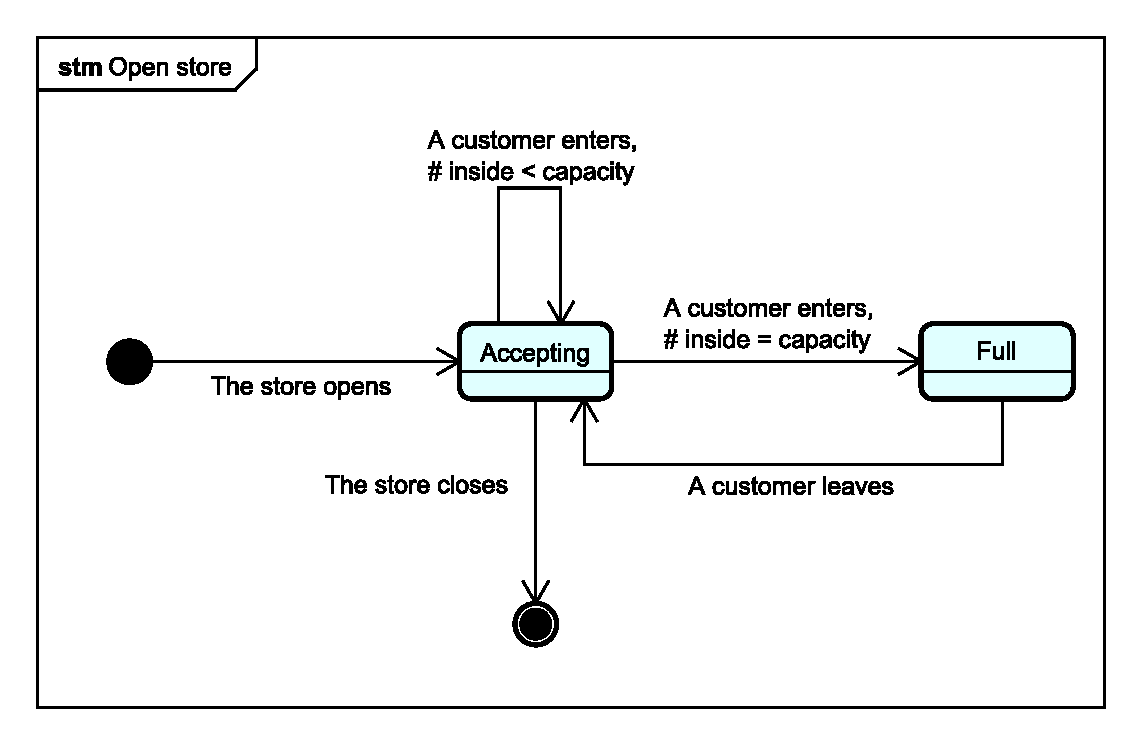
\includegraphics[width=0.9\textwidth] {state_diagrams/open_store}
		\caption{Open store diagram}
		\label{open_store} 
	\end{figure}
\end{center}

\begin{landscape}
	\begin{figure}[hp]
		\centering	
		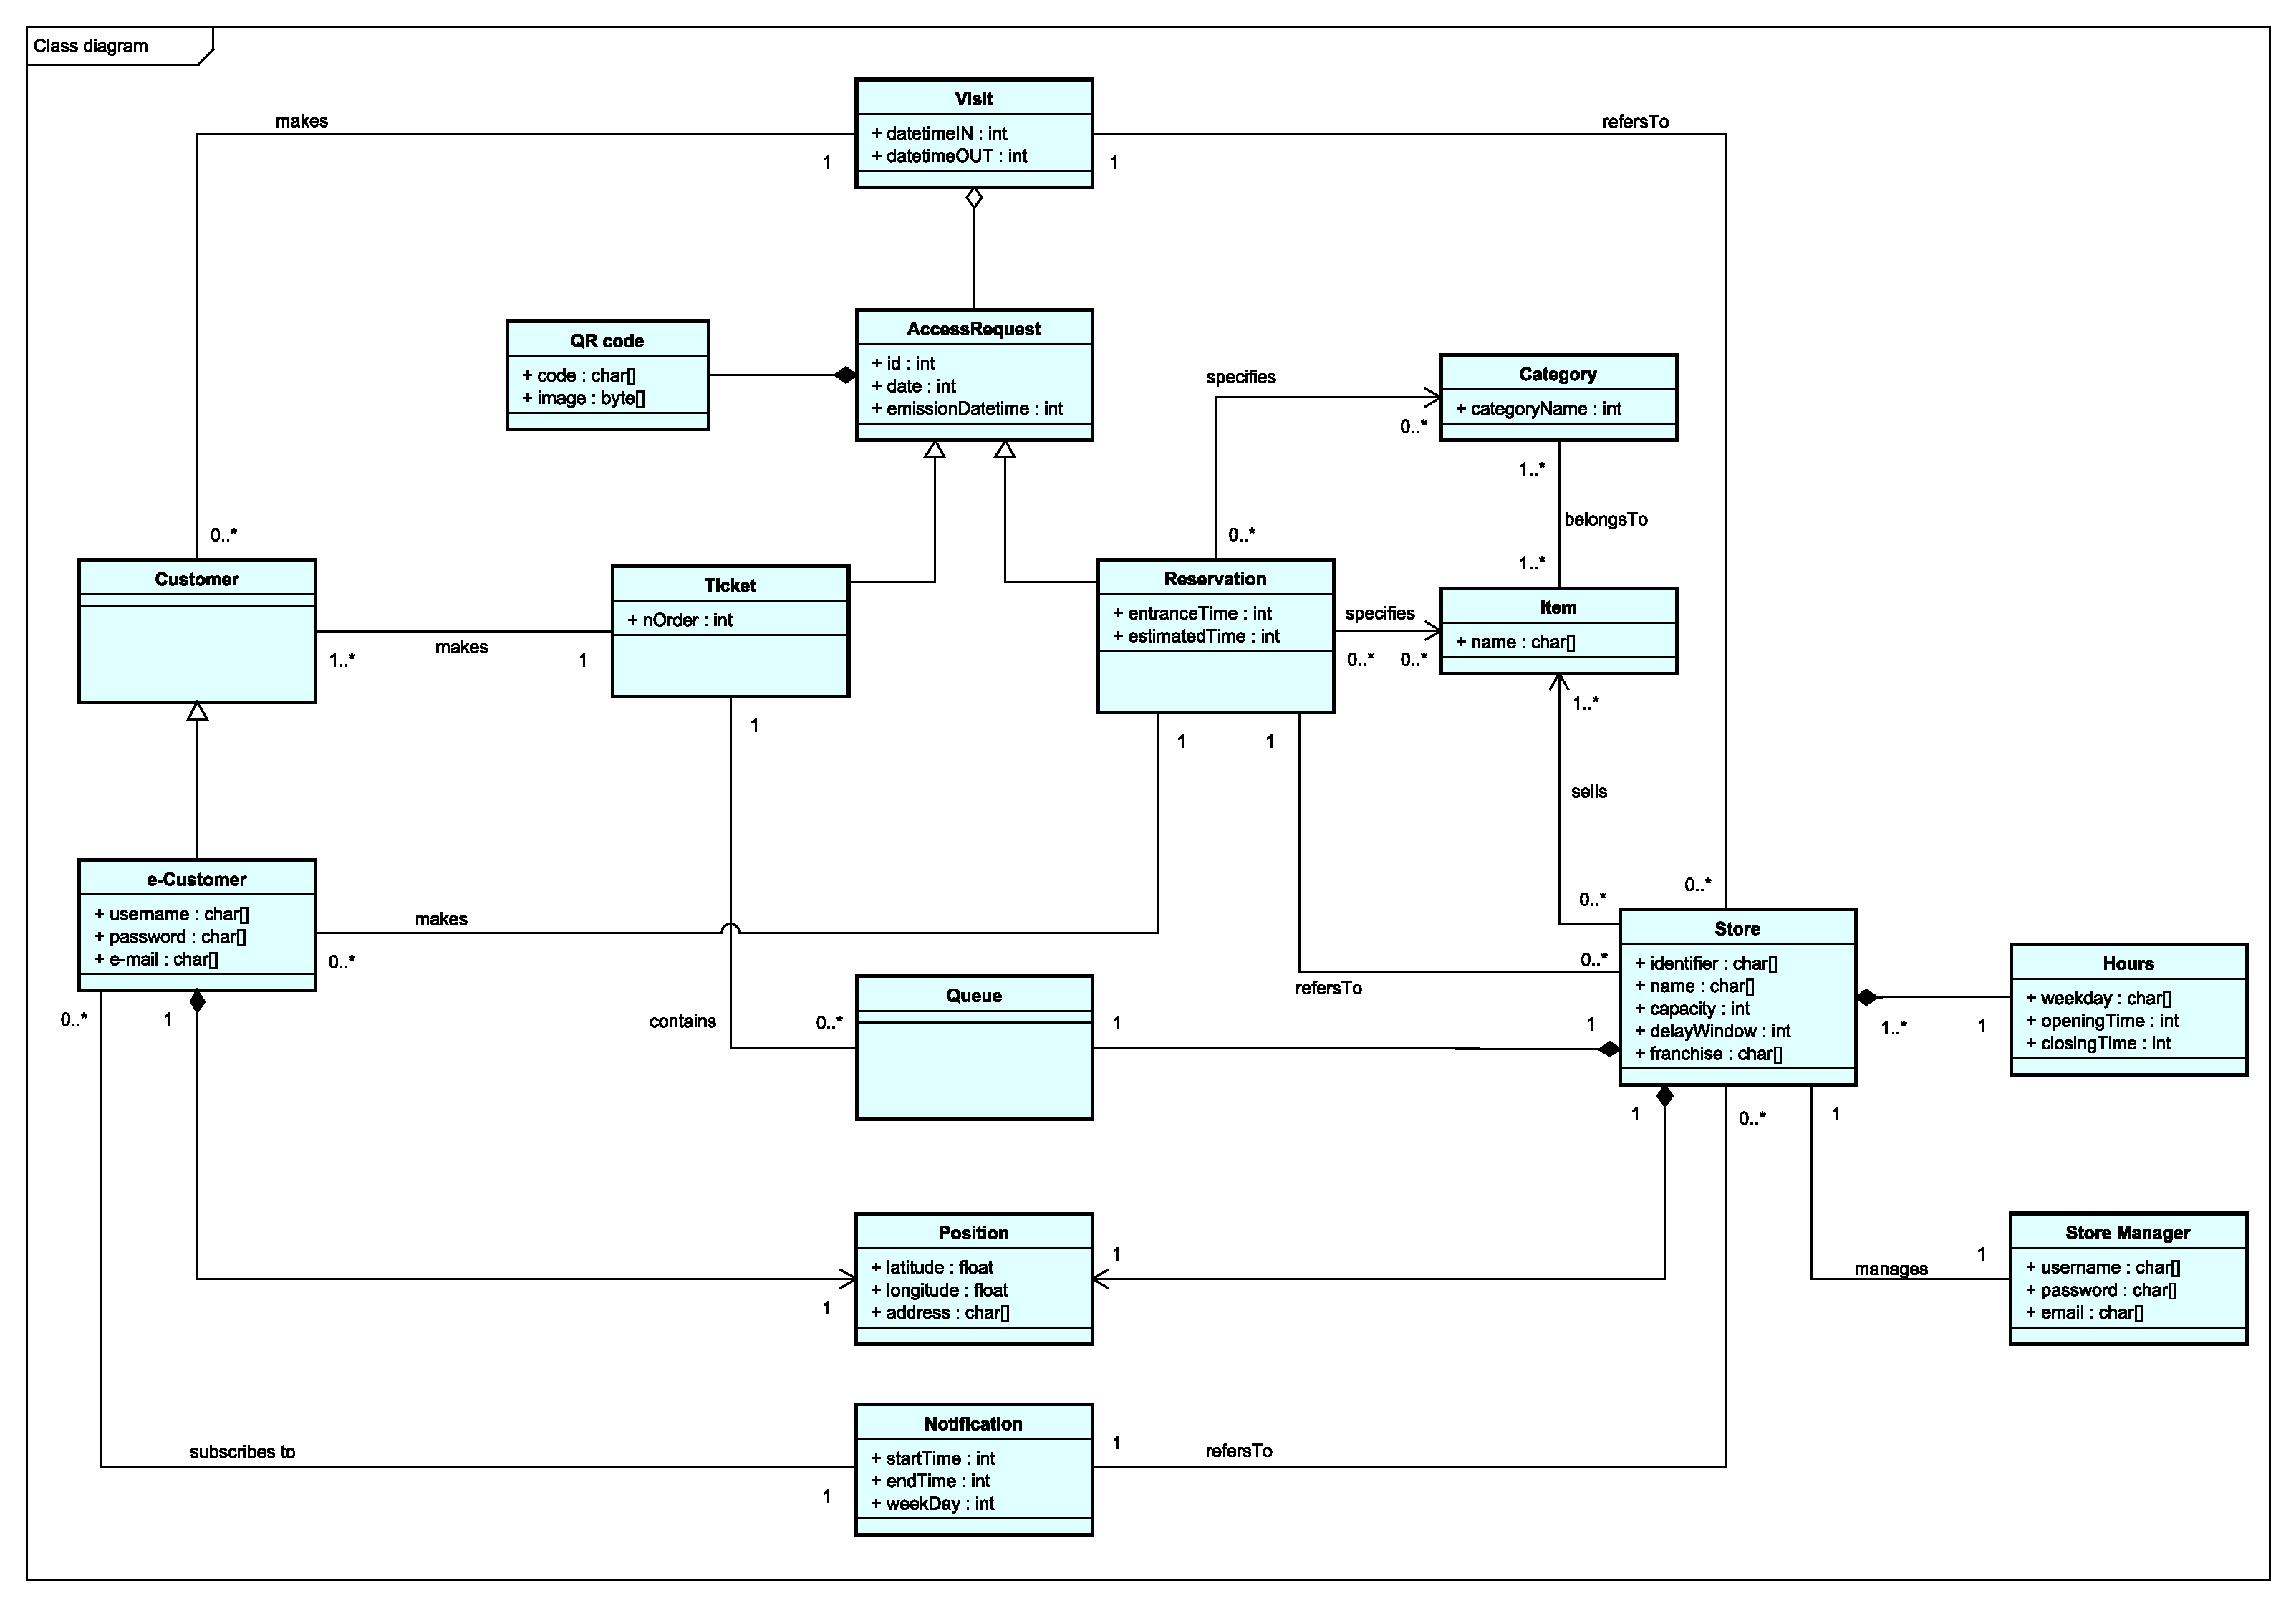
\includegraphics[height=\textheight] {class}
		\caption{Class Diagram}
		\label{class} 
	\end{figure}
\end{landscape}
